
\begin{frame}
		\frametitle{ Different possible swapping strategies $p_{ij}( x )$ }

	\begin{itemize}
		\item[] Strategy I 
		\item[] 
	$$p_{ij}(x) \propto \frac{\pi (x_j)}{\pi( x_i )} \wedge \frac{\pi (x_i)}{\pi( x_j )} = \exp \Big( - | \log ( \pi(x_j) ) - \log ( \pi(x_i) ) | \Big)$$
		\begin{itemize}		
 			\item promotes swaps between coordinates relatively the same,  $\pi (x_j) \approx \pi (x_i)$ 
		\end{itemize}
	
		\item[] Strategy II 
		\item[] 
	$$p_{ij}(x) \propto \frac{\pi (x_j)}{\pi (x_i)} \wedge 1 = \exp \Big( - ( \log ( \pi(x_j) ) - \log ( \pi(x_j) ) )\Big) \wedge 1$$
		\begin{itemize}		
 			\item breaks the symmetry of the previous one
		\end{itemize}

	\end{itemize}

\end{frame}

	% Strategy One
\begin{frame}[plain]

	\begin{center}
		\begin{figure}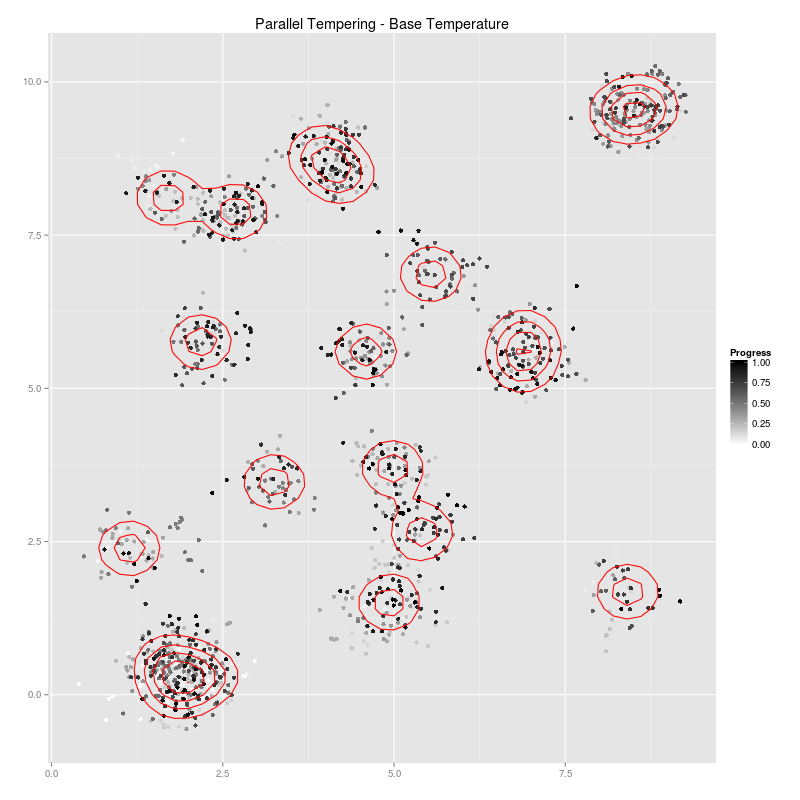
\includegraphics[scale=.31]{./picts/PT_simululation_base_temperature_2000_steps_strategy_1_try_1.png}\end{figure}	
	\end{center}	
		
\end{frame}


	% Strategy Two
\begin{frame}[plain]

	\begin{center}
		\begin{figure}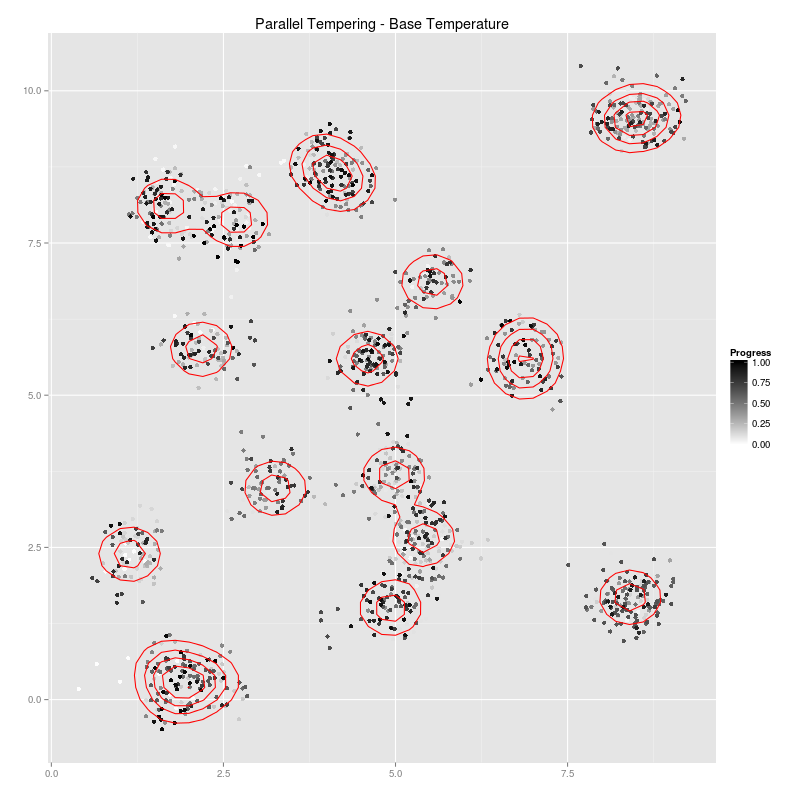
\includegraphics[scale=.31]{./picts/PT_simululation_base_temperature_2000_steps_strategy_2_try_1.png}\end{figure}	
	\end{center}	
		
\end{frame}


%%%%%%%%%%%%%%%%%%%%%%%%%%%%%%%%%%%%%%%%%%%%%%%%%%%%%%%%%%%%%%%%%%%%%
\begin{frame}
		\frametitle{ Different possible swapping strategies $p_{ij}( x )$ }

	\begin{itemize}
		\item[] Strategy III 
		\item[] 
	$$p_{ij} \propto \Big( \frac{\pi (x_j)}{\pi( x_i )} \wedge \frac{\pi (x_i)}{\pi( x_j )} \Big)^{\beta_i - \beta_j} = \exp \Big( - (\beta_i - \beta_j)| \log ( \pi(x_j) ) - \log ( \pi(x_i) ) | \Big)$$
		\begin{itemize}		
 			\item softens the requirement  $\pi (x_j) \approx \pi (x_i)$
			\item promotes $\beta_i - \beta_j \approx 0$ 
			\item promotes swaps between adjacent chains 
		\end{itemize}
	
		\item[] Strategy IV 
		\item[] 
	$$p_{ij} \propto \Big( \frac{\pi (x_j)}{\pi( x_i )} \wedge \frac{\pi (x_i)}{\pi( x_j )} \Big)^\frac{\beta_i - \beta_j}{1 + \rho(x_i, x_j)} = \exp \Big( - \frac{(\beta_i - \beta_j)| \log ( \pi(x_j) ) - \log ( \pi(x_i) ) |}{{1 + \rho(x_i, x_j)}} \Big)$$
		\begin{itemize}		
 			\item added a quasi-metric 
			\item $\rho$ does not require symmetry $\rho(x_i, x_j) = \rho(x_j, x_i)$  
			\item could be of use in the Gibbs random-field model
		\end{itemize}

	\end{itemize}

\end{frame}

	% Strategy Three

\begin{frame}[plain]

	\begin{center}
		\begin{figure}\includegraphics[scale=.31]{./picts/PT_simululation_base_temperature_2000_steps_strategy_3_try_1.png}\end{figure}	
	\end{center}	
		
\end{frame}

	% Strategy Four

\begin{frame}[plain]

	\begin{center}
		\begin{figure}\includegraphics[scale=.31]{./picts/PT_simululation_base_temperature_1000_steps_1.png}\end{figure}	
	\end{center}	
		
\end{frame}

\begin{frame}[plain]

	\begin{center}
		\begin{figure}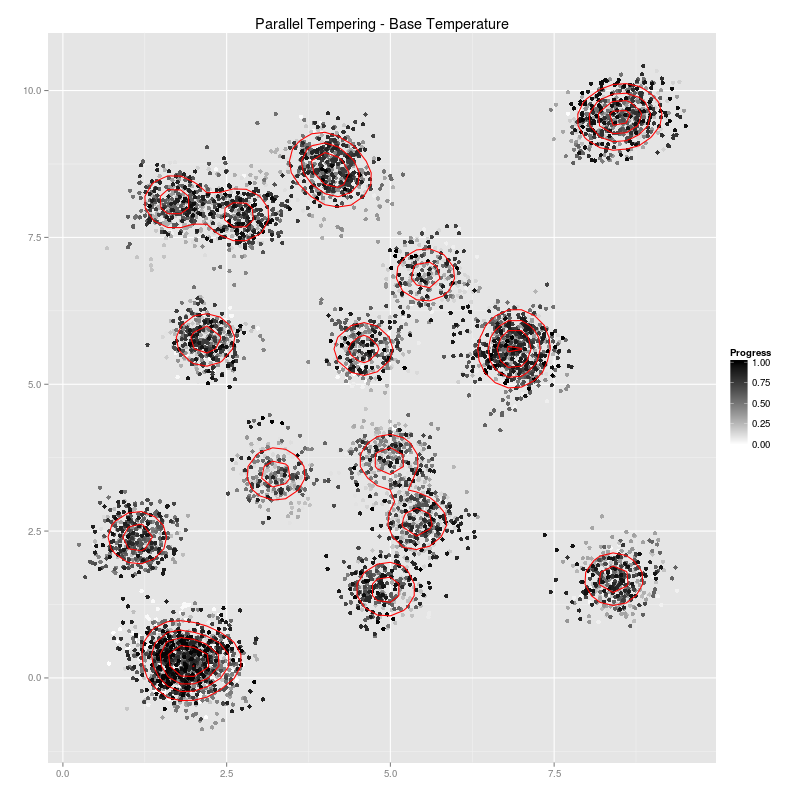
\includegraphics[scale=.31]{./picts/PT_simululation_base_temperature_10000_steps_1.png}\end{figure}	
	\end{center}	
		
\end{frame}




